\chapter{Introduction}

The context project is a project in which bachelor students at the TU Delft should develop a product in 10 weeks.
Our clients from the business world want this product to be developed.

The task we were assigned to was to design the music services of tomorrow.
Our group had to design an application that would allow users to listen to music of a certain mood and interact with people in the same mood.


The system should allow users select a mood and a room, where after they join a room according to the selected mood.
When a user is logged in, he should be able to send messages to other users in the room.
Additionally a user can classify a song according to mood of the song.
Lastly there should be a ranking game where users can classify unranked songs.
The user shall be rewarded with points for contributing to the system.


In this report we will explain MoodCat and how we have developed this system.
First we will give an overview of the overall system and secondly reflect on the product and process.
Thirdly we will explain the different functionalities of MoodCat After that we will elaborate the interaction between the user and our system.
Then we will evaluate the functionalities and provide a list of implemented features.
Lastly we will give an outlook of possible improvements for the system and how they could be implemented.\\

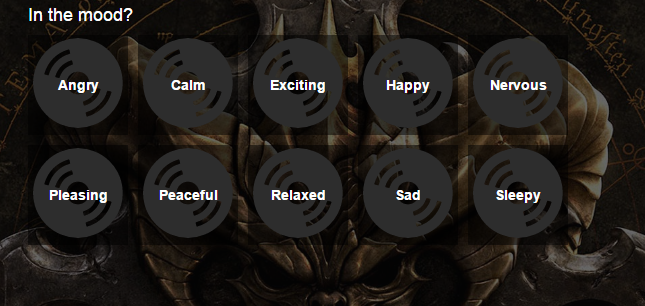
\includegraphics[width= 0.75\textwidth]{moodselection.png}